\section{Methoden}

\begin{frame}\frametitle{Inhalt}
	\tableofcontents[currentsection,hideallsubsections]
\end{frame}

\subsection{Zeitdiskretes Survival-Modell}

\begin{frame}
	\begin{itemize}
		\item Zeit bis zu einem Ereignis $\Rightarrow$ Konvertierung oder Nicht-Konvertierung bzw. Rechtszensierung
		\item Positionen bilden Zeitachse des Modells $\Rightarrow$ Zeitdiskretes Modell
		%\item Stochastic Gradient Boosting mit Stümpfen als Basis-Lerner
		\item Zielvariable:	
			\begin{align*}
				y_{ip} =& \begin{cases} 1 & \text{Beobachtung } i \text{ konvertiert an Position } p\\
															 0 & \text{sonst} 
								 \end{cases}\\
								&p=1,...,25 \text{, } i=1,...,N_p 
			\end{align*}	
	\end{itemize}
\end{frame}

\begin{frame}
	\begin{itemize}
		%\item Zielvariable:	
			%\begin{align*}
				%y_{ip} =& \begin{cases} 1 & \text{Beobachtung } i \text{ konvertiert an Position } p\\
					%										 0 & \text{sonst} 
						%		 \end{cases}\\
							%	&p=1,...,25 \text{, } i=1,...,N_p 
			%\end{align*}	
		\item Hazardrate: 
			\begin{align*}
				\lambda_{ip} = P(y_{ip}=1|funnelLength_i \geq p, x_{ip})
			\end{align*}
		\item Logit-Modell: 
			\begin{align*}
				y_{ip}|x_{ip} &\stackrel{ind}{\sim} Bin(1, \lambda_{ip})  \\
				E(y_{ip}|x_{ip}) = P(y_{ip} = 1|x_{ip}) = \lambda_{ip} &= h(f_p(x_{ip})) = \frac{\exp(f_p(x_{ip}))}{1+\exp(f_p(x_{ip}))}
			\end{align*}
		\item Binomieller Verlust: 
			\begin{align*}
				L(y_{ip},f_p(x_{ip})) = -\sum_{i=1}^{N_p} (y_{ip} f_p(x_{ip}) + \ln(1+\exp(f_p(x_{ip}))))
			\end{align*}
	\end{itemize}
\end{frame}

%\begin{frame}
	%\begin{itemize}
		%\item Likelihood: 
			%\begin{align*}
				%L(\lambda_{ip}) &= \prod_{i=1}^{N_p} \lambda_{ip}^{y_{ip}} (1-\lambda_{ip})^{1-y_{ip}}
			%\end{align*}
		%\item Log-Likelihood: 
			%\begin{align*}
				%l(\lambda_{ip}) &= \ln(L(\lambda_{ip})) = \sum_{i=1}^{N_p} (y_{ip} \ln(\lambda_{ip}) + (1-y_{ip}) \ln(1-\lambda_{ip}))\\
				%&= \sum_{i=1}^{N_p} (y_{ip} f(x_{ip}) - \ln(1+\exp(f(x_{ip}))))
			%\end{align*}
		%\item Binomieller Verlust: 
			%\begin{align*}
				%L(y,f) = -yf + \ln(1+\exp(f))
			%\end{align*}
	%\end{itemize}
%\end{frame}

\begin{frame}
	\begin{itemize}
		\item Prädiktorfunktion:
			\begin{align*}
			f_p(x_{ip}) =&f_{weekday,p}(\text{weekday}_{ip}) +\\
								 &f_{hour,p}(\text{hour}_{ip}) +\\
								 &f_{campaign,p}(\text{campaign}_{ip}) +\\
								 &f_{campaignLast,p}(\text{campaign}_{i,p-1}) +\\
								 &f_{campaignLast2,p}(\text{campaign}_{i,p-2}) +\\
								 &f_{timeSinceLast,p}(\text{timeSinceLast}_{ip}) +\\
								 &f_{timeSinceFirst,p}(\text{timeSinceFirst}_{ip}) +\\
								 &\text{offset}(\hat{\lambda}_{i,p-1})
			\end{align*}
	\end{itemize}
\end{frame}

\begin{frame}\frametitle{Gradient Boosting - Pseudocode}
	\floatname{algorithm}{Algorithmus}
	%\begin{algorithm}
	%\caption{Gradient Boosting}\label{alg}
	%\label{gradboosting}
		\begin{algorithmic}
		\STATE Setze Startwert für $f_{0p}(x_{ip})$
		\FOR{$m=1:n.trees$}
			\STATE Setze $\lambda_{ip}(x_{ip}) = \frac{\exp(f_{m-1,p}(x_{ip}))}{1+\exp(f_{m-1,p}(x_{ip}))}$
			\FOR{$i=1:N_p$} 
				\STATE $r_{imp} = - \frac{\partial L(y_{ip},f_{m-1,p}(x_{ip}))}{\partial f_{m-1,p}(x_{ip})} = y_{ip} - \lambda_{ip}(x_{ip})$
			\ENDFOR
			%\STATE Fit a regression base learner to the pseudo-residuals $r_{im}$:
			\STATE $\theta_{mp} = \argmin_{\theta} \sum_{i=1}^{N_p} (r_{imp} - h(x_{ip}, \theta))^2$
			\STATE $\beta_{mp} = \argmin_{\beta} \sum_{i=1}^{N_p} L(y_{ip}, f_{m-1,p}(x_{ip}) + \beta h(x_{ip},\theta_{mp}))$
			\STATE $f_{mp}(x_{ip}) = f_{m-1,p}(x_{ip}) + \beta_{mp} h(x_{ip},\theta_{mp})$
		\ENDFOR
		\end{algorithmic}
	%\end{algorithm}
\end{frame}

\begin{frame}\frametitle{Parameter des Modells}
	\begin{itemize}
		\item Trainingsdaten machen Hälfte der gesamten Daten aus - stratifiziert bezüglich Transaction, Campaign, funnelLength
		\item $n.trees=3000$
		\item $cv.folds=5$
		\item Shrinkage-Parameter: $\mu = 0.01 \Rightarrow f_{mp}(x_{ip}) = f_{m-1,p}(x_{ip}) + \mu \beta_{mp} h(x_{ip},\theta_{mp})$
		\item $interaction.depth=1$
		\item $bag.fraction=0.5 \Rightarrow$ \textbf{Stochastic} Gradient Boosting
	\end{itemize}
\end{frame}

\begin{frame}\frametitle{Output des Modells}
	\begin{itemize}
		\item $\hat{f}_p(x_{ip})$ für jede Beobachtung $i$ und jede Position $p$
			\begin{align*}
				\hat{\lambda}_{ip} = \frac{\exp(\hat{f}(x_{ip}))}{1+\exp(\hat{f}(x_{ip}))}
			\end{align*}
		\item Relative Wichtigkeit der Features:
			\begin{align*}
				\hat{I}_{jp} &= \sqrt{\frac{1}{M} \sum_{m=1}^{n.trees} \hat{i}_{mp} 1_{jmp}}
			\end{align*}
		\item Marginale Effekte der Features:
			\begin{align*}
				\bar{f}_{jp}(x_{jp}) = \frac{1}{N} \sum_{i=1}^{N_p} \hat{f}(x_{jp},x_{i,\backslash j,p})
			\end{align*}
		\item ROC-Kurve und AUC
	\end{itemize}
\end{frame}

\subsection{Sequential Pattern Mining}

\begin{frame}
	\begin{itemize}
		\item Menge von Items $I = \{a, b, c, d, e\}$ $\Rightarrow$ Kampagnen
		\item Datenbank: $[ID 1, <abcdbaae>]$; $[ID 2, <edcaa>]$
		\item 4-Sequenz $s = b\rightarrow b\rightarrow a\rightarrow e$
		\item Support einer Sequenz: Anteil der IDs, die $s$ unterstützen
		\item SPADE-Algorithmus findet häufige Sequenzen, deren Support größer als ein festgelegter minimaler Support ist
		\item Seperate Anwendung auf konvertierte und nicht-konvertierte Funnels
	\end{itemize}
\end{frame}

\subsection{Visualisierung anhand eines Netzwerkes}

\begin{frame}
	\begin{itemize}
		\item Geordneter Graph $G=(V,E)$ besteht aus Menge $V$ von Knoten und Menge $E$ von Kanten
		\item Kante $e_i \in E$ besteht aus geordneten Paar von zwei Knoten $(v_j,v_k)$, wobei $v_j,v_k \in V$
		\item Startpunkt $\rightarrow$ $17$ Kampagnen der ersten Position $\rightarrow$ $Succ\_1$, $Fail\_1$ und $17$ Kampagnen der zweiten Position $\rightarrow$ $Succ\_2$, $Fail\_2$ und $17$ Kampagnen der dritten Position $\rightarrow$ ...
		\item Kanten sind bezüglich der Anzahl der Nutzer gewichtet
		\item Relative Ausgänge: relative Häufigkeiten der Kanten, wobei die zugrundeliegende Menge die Summe aller Nutzer ist, die einen Knoten verlassen
		\item Relative Eingänge: relative Häufigkeiten der Kanten, wobei die zugrundeliegende Menge die Summe aller Nutzer ist, die in einen Knoten gehen
	\end{itemize}
\end{frame}

\begin{frame}
	\begin{itemize}
		\item \textit{R}-Paket \textit{rgexf} $\rightarrow$ \textit{gexf}-Datei $\rightarrow$ \textit{Gephi}
		\item Berechnung der räumlichen Anordnung der Knoten und Kanten anhand von Algorithmen (z.B. \textit{Force Atlas 2})
		\item Manuelle Bearbeitung für die Präsentation von Ergebnissen
		\item Interaktives Arbeiten mit dem Netzwerk in \textit{Gephi} möglich $\rightarrow$ Tutorial dazu im Bericht
	\end{itemize}
	\centering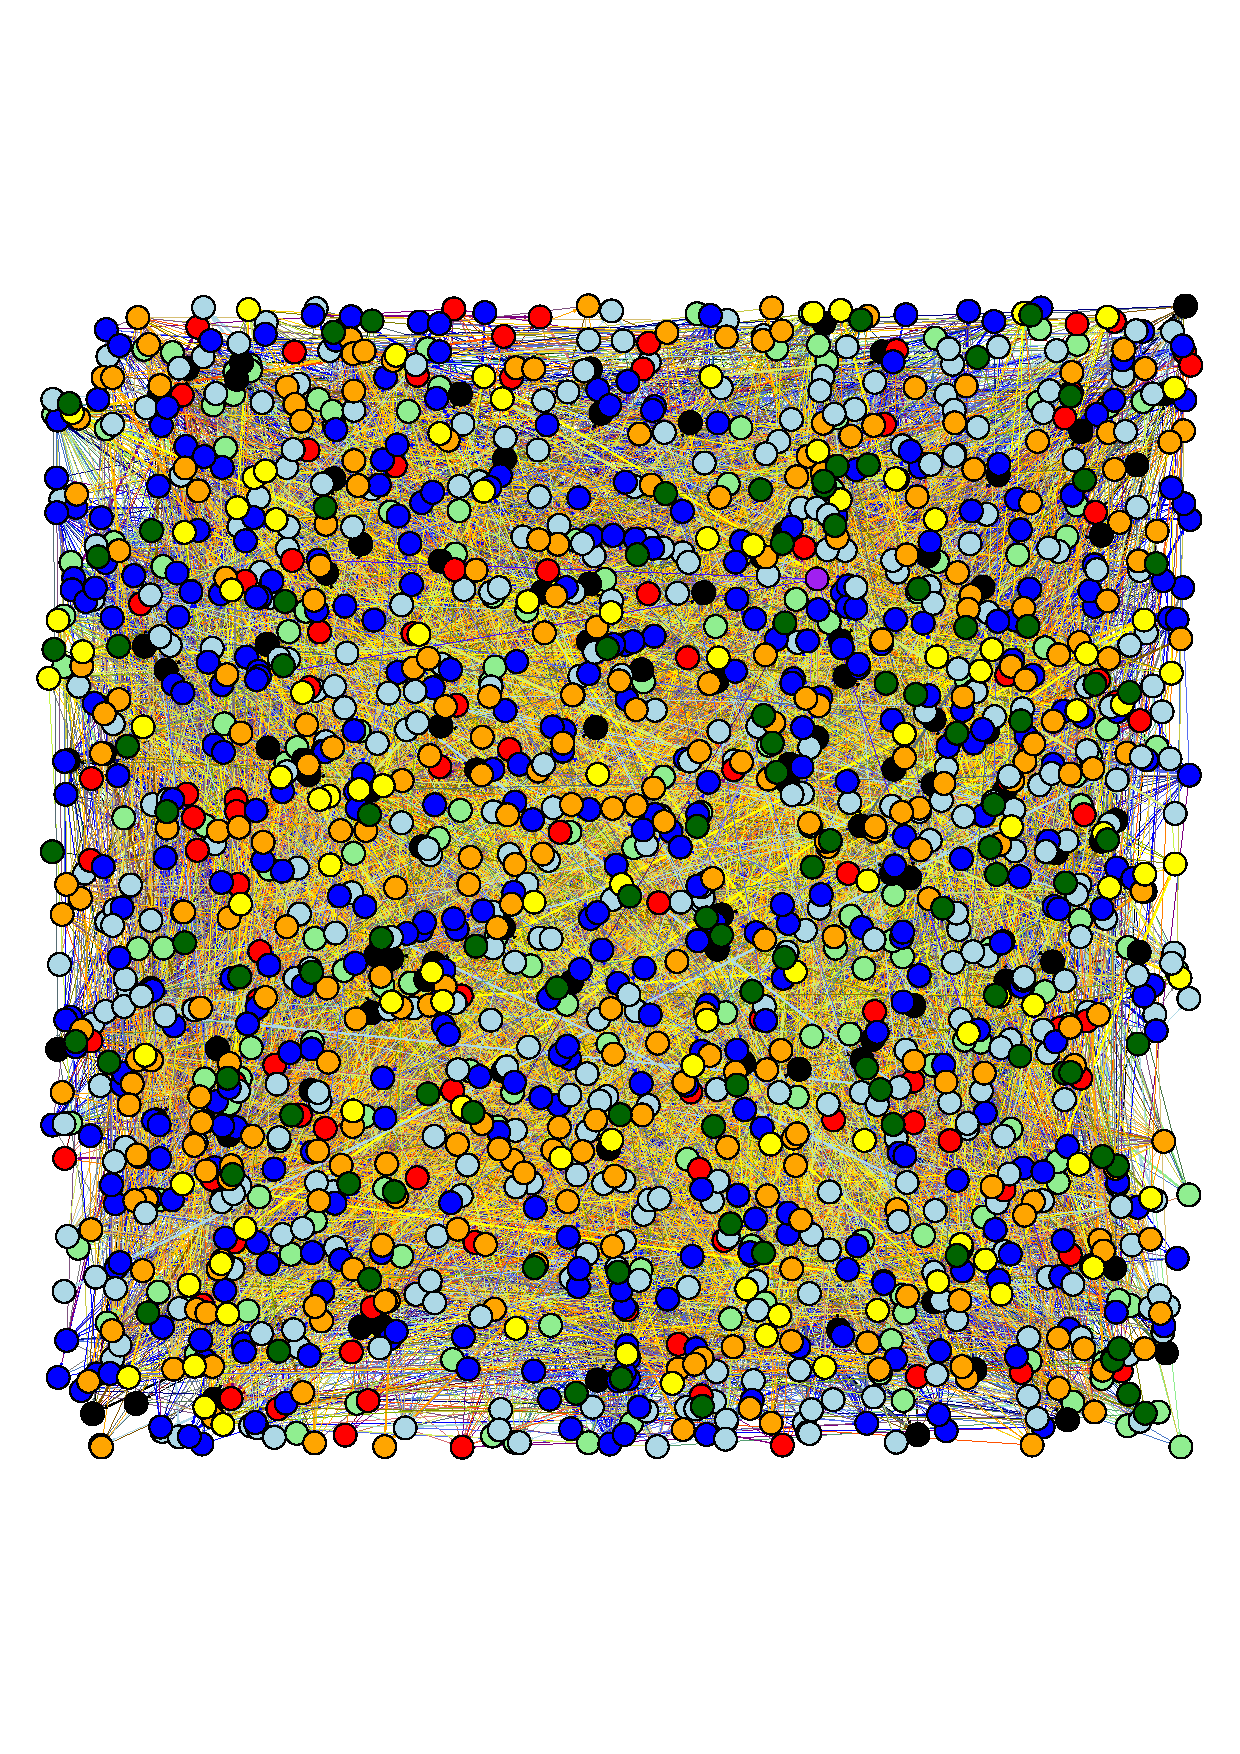
\includegraphics[scale=0.2]{graphbegin.pdf}
\end{frame}
